\chapter{The NLogN algorithm}
In this chapter we will walk through the $O(nlogn)$ algorithm for the MAST problem described in the paper \cite{nlogn} by Cole et. al. We will give a detailed description of each step of the algorithm and analyse its time complexity and space consumption.

\begin{figure}
	$T_1:$ \Tree [.A [.B [.C 3 7 ] [.D 0 5 ] ].B [.E [.F 2 1 ] [.G 4 6 ] ].E ].A
	$T_2:$ \Tree [.H [.I [.J 0  1 ] [.K 2 3 ] ].I [.L [.M 4 5 ] [.N 6 7 ] ].L ].H
	
	\caption{Two example input trees}
	\label{Fig:InputTrees}
\end{figure}

\section{Definitions and Notations}
\subsubsection{Trees}
In the rest of the chapter, all trees will be binary rooted trees \todo{$log$ means $log_2$} \todo{also the case for other chapters - move to introduction?}. The size of a tree is the number of leaves, and for a tree $T$, $T(x)$ will refer to the subtree of $T$ having $x$ as root. We will refer to the two input trees as $T_1$ and $T_2$ each of which have size $n$. Every leaf of $T_1$ has a unique name and for each of these leaves there is a corresponding leaf in $T_2$ with that same name. These two leaves are said to be twins.

\subsubsection{Centroid Decompositions}
The centroid decomposition for $T_1$ is a path of nodes $u_1, u_2, ..., u_p$ in the tree, starting from the root and ending at a leaf. Such a path is called a centroid path. It is referred to as $\pi$ and has length $p$.

The centroid decomposition for $T_2$ is a set of disjoint centroid paths in the tree. The node in each path closest to the root of $T_2$ is referred to as the start node and $\pi(x)$ is the path having the node $x$ as its start node. $X$ will refer to the set of start nodes in the centroid decomposition for $T_2$.

Each node $v$ in a centroid path has a side tree, which is the subtree having as root the child of $v$ which is not on the centroid path. If $v$ is a leaf, the side tree is $v$ itself. The side tree of a node $u_i$ in $\pi$ is referred to as $M_i$ and has size $m_i$. The side tree of a node $v_j$ in a path $\pi(x)$ is referred to as $N_j$ and has size $n_j$. Figure \ref{centroidFigure} illustrates the principle of centroid paths in $T_1$ and $T_2$.

\begin{figure}
	\label{centroidFigure}
	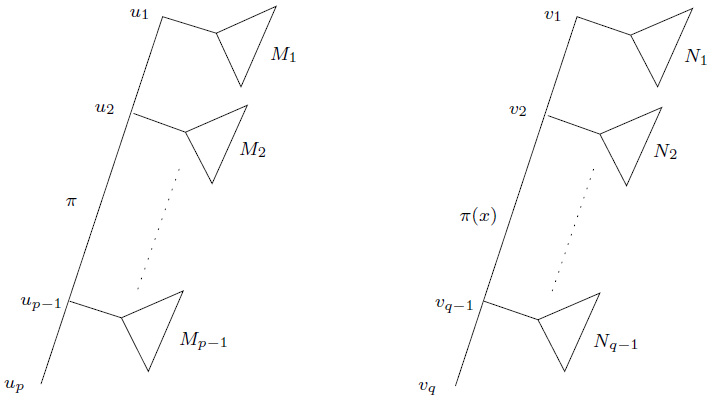
\includegraphics[width=\textwidth]{CentroidDecompositions}
	\caption{Centroid paths in $T_1$ and $T_2$ with $\pi$ starting in root of $T_1$ and $\pi(x)$ starting in $x = v_1$ in $T_2$. \cite{nlogn}}
\end{figure}

Given a side tree $M_i$ of $\pi, 1 \le i \le p-1$, $S_i$ will refer to the subtree of $T_2$ induced by the leaves in $T_2$ corresponding to the leaves in $M_i$.

\section{The Overall Strategy}
The idea of the algorithm is that an Agreement Subtree $A$ can be represented as a bipartite graph, where each edge represents a distinct subtree of $A$ and the weight of the edge is the size of that subtree. This special kind of graph, called an Agreement Matching is defined in a way that makes sure that it satisfies everything that an Agreement Subtree should satisfy. The purpose of the algorithm is now to compute the Largest Weight Agreement Matching (LWAM) for two input trees $T_1$ and $T_2$, which in the end can be translated to the Maximum Agreement Subtree. It will be a requirement that the two input trees contain the exact same leaves.

The algorithm '$computeLWAM(T_1,T_2)$' has five overall steps, each of which will be covered in the following sections.

\begin{enumerate}
	\item Create centroid decompositions.
	\item Induce subtree $S_i$ of $T_2$ from each side tree $M_i$ of $\pi$.
	\item Recursively construct $computeLWAM(M_i, S_i), 1 \le i \le p-1$.
	\item Create a Matching Graph for each path $\pi(x)$ in the decomposition of $T_2$.
		\subitem A Matching Graph is a bipartite graph used to compute the Agreement Matchings.
	\item Compute Agreement Matchings and find the Largest Weight Agreement Matching.
\end{enumerate}

\section{Initial Setup}
One thing we need to set up before starting the main algorithm, is to make sure that from any leaf in either $T_1$ or $T_2$, its twin in the other tree can be found in constant time. Note that this only needs to be done at the beginning of the algorithm and not for every recursive call.

First we want the names of all leaves to be numbers from 0 to $n-1$. This is done before starting the algorithm, e.g. when reading the input trees. Of course it should be possible to obtain the original names from the new names after the algorithm has finished, so one could for example store the original names in a list at indices corresponding to the new names.

Setting up twins is done by storing a list containing the leaves of $T_2$, where each leaf is at the index corresponding to its name, the twin of a leaf named $i$ from $T_1$ can be looked up in constant time from the list for $T_2$ at index $i$. Then the twins of all leaves can be set in $O(n)$ time.

\section{Centroid decompositions}
The first step of the algorithm is to compute the \texttt{Centroid decomposition}s for the two trees. Recall that a centroid decomposition consists of one or more disjoint centroid paths through the tree. The first path starts at the root node in the tree. The next node is the child node holding the largest amount of leaves in its subtree and so forth. In case of a tie, we will pick the left node, but either one of the children could be picked. The path will continue until reaching a leaf.

For $T_1$, this is the only path in the centroid decomposition. For $T_2$, there is a new path starting at the root of each side tree if it is not a leaf, such that all internal nodes of $T_2$ is in a centroid path.

Creating the centroid decompositions can be done in $O(n)$ time in the following way:

First, at each node $v$ in the two trees we need to store the number of leaves in the subtree having $v$ as root. This can be done in a single post-order traversal of each tree. For a leaf, the number is 1. For an internal node, it is the sum of the numbers stored at its two children. Clearly this takes $O(n)$ time.

Now for the centroid decomposition of the first tree, we simply start with the root node and add the child node with the highest number stored. For the second tree, the same thing is done, but when adding a child node, another path is started at the child that wasn't added if it's not a leaf. While creating the paths for $T_2$ we will make each node on a path point to the start node of that path. This will be useful later in the algorithm.

Each node is not visited more than once so the time complexity is $O(n)$.

\section{Induced subtrees of $T_2$}
Having created the centroid decompositions, the second step of the algorithm is to compute the induced subtrees of $T_2$ from each side tree of $\pi$. Given a side tree $M_i$ of $\pi$, the induced subtree $S_i$ of $T_2$ is the subtree containing only leaves that are twins of the leaves in $M_i$. Take figure \ref{Fig:InputTrees} as an example. Let the side tree $M_i$ be the subtree of $T_1$ with $E$ as the root. Then $S_i$ is the subtree having only the leaves named $1, 2, 4$ and $6$ as shown in figure \ref{Fig:InducedSubtree}. 

\begin{figure}
	\Tree [.H [.I 1 2 ] [.L 4 6 ] ].H
	\caption{The subtree induced from $T_1(E)$ in figure \ref{Fig:InputTrees}}
	\label{Fig:InducedSubtree}
\end{figure}

Given a tree $T$ and an ordered set of leaves, $L=l_1,l_2,l_3,...,l_{|L|}$, we will show how the subtree induced by $L$ can be computed in $O(|L|)$ time after having preprocessed $T$ in $O(|T|)$ time.

\subsection{Preprocessing}
To induce the subtree of $T$ from $L$ in $O(|L|)$ time, two requirements must be met.
\begin{enumerate}
	\item The depth of any node in $T$ can be retrieved in constant time.
	\item The Least Common Ancestor (LCA) between two leaves can be computed in $O(1)$ time.
\end{enumerate}

Both of these requirements can be achieved in $O(|T|)$ time.

The node depths can be set in $O(|T|)$ time by a simple pre-order tree traversal, where the depth of each node is set to its parent's depth plus one. The depth of the root is initialized to zero.  

Computing LCA in $O(1)$ time is possible after having preprocessed $T$ in $O(|T|)$ time. This is however a more complicated matter, and is covered in section \ref{lcaSection}.

\subsection{Inducing the subtree}
The algorithm works in 3 steps:
\begin{enumerate}
	\item Find the LCA of each consecutive pair of leaves and add them to $L$ such that $LCA(l_i,l_{i+1}), 1 \le i \le |L|-1$ is added between $l_i$ and $l_{i+1}$.
	\subitem After this step, $L$ will contain all nodes in the induced subtree.
	\subitem We will refer to the modified $L$ as $L'$.
	\item For each node $v$ in $L'$, find the closest node on either side, $v_l$ and $v_r$, that has smaller depth than itself.
	\item Construct the tree: The parent of each node $v$ will be whichever of $v_l$ and $v_r$ that has the greatest depth.
\end{enumerate}

Since the LCA between two leaves can be computed in constant time, the first step takes $O(|L|)$ time.

The challenge was to perform step 2 in linear time, which is not covered by Cole et. al \cite{nlogn}. We did this by realizing that for any node $v$ in $L'$ that has greater depth than the node immediately to the right of it in $L'$, $v_l$ and $v_r$ are the nodes immediately to the left and right in $L'$ (because of how the LCAs were added to the set). By not considering these nodes any more, the same will be the case for the nodes that now has greater depth than the node to the right of it in $L'$. This resulted in the approach for step 2 seen in listing \ref{lst:induceSubtreeCode}. Here, each node $v$ of $L'$ will eventually be added to $S$ and removed when $v_l$ and $v_r$ has been updated correctly. For each node, a constant amount of computation needs to be performed, so the time complexity is $O(|L'|) = O(|L|)$.

Step three is done in a single iteration through $L'$ where the parent of each node is found in constant time, giving a total runtime of $O(|L'|) = O(|L|)$.

\begin{lstlisting}[language=Java, caption=Step 2 of induceSubtree, label={lst:induceSubtreeCode}]
Function induceSubtree(inputLeaves)
{
	...
	
	L` = The list of nodes computed in step 1;
	for each node v in L`
		v_l = the node to the left of v in L`;
		// if v is the leftmost node in L`, v_l = null
		v_r = the node to the right of v in L`;
		// if v is the rightmost node in L`, v_r = null
	S = Stack initially containing only the first node in L`;

	while(S is not empty)
	{
		v = S.peek();
		if(v_r == null || depth(v) > depth(v_r))
		{
			remove v from S;
			if(v_l != null) (v_l)_r = v_r;
			if(v_r != null) (v_r)_l = v_l;
			
			if(S is empty) push v_r on S;
		}
		else
			push v_r on S;
	}

	...
}
\end{lstlisting}

\subsection{Computing the induced subtrees of $T_2$}
Now that we can induce a subtree from a set of leaves $L$ in $O(|L|)$ time, all we need is to find the leaves from which we can induce the subtree $S_i$ of $T_2$, given the subtree $M_i$.

In order to induce subtree $S_i$, the input leaves needs to be sorted by the order that they appear in $T_2$. Our approach to this is to first compute a sorted list of all leaves in $T_1$ according to $T_2$, then splitting the leaves into lists corresponding to the subtrees $M_i$, $1 \le i \le p-1$ and finally use their twins (which can be found in constant time) to induce the subtree $S_i$ for each list.

The leaves of $T_1$ is sorted by first giving each leaf of $T_2$ a number corresponding to its position (left to right) in $T_2$. This is done by a single iteration through $T_2$. Then we sort the leaves from $T_1$, by looking up the number of its twin in $T_2$, in linear time using bucket sort.

%For the input trees, the leaves of $T_1$ could also be sorted by their name, assuming that the names of $T_2$ where sorted. However, in the recursive calls the names will no longer correspond to the number of leaves, meaning that they can't be sorted in linear time. Therefore we instead assign numbers to the leaves of $T_2$.

% First try
% Creating a list, where index $i$ holds the position, left to right, of the leaf named $i$ in $T_2$ compared to the other leaves, is done in linear time simply by iterating through $T_2$. That list is used when sorting the leaves of $T_1$ to look up the position of the twins in $T_2$. We sort the leaves in linear time using bucket sort.

By iterating through each subtree $M_i$, we can use linear time to have each leaf store a number corresponding to the subtree to which it belongs. Having the sorted list of leaves in $T_1$, we can use the stored numbers to split the leaves into the final lists during a single iteration. Now the twins can be found and the subtrees $S_i$, $1 \le i \le p-1$ can be computed.

In our implementation, $S_i$ does not actually consist of nodes from $T_2$. It is a new tree where each node contains a reference to the corresponding node in $T_2$ and vice versa.

\subsection{Time Complexity}
First, $T_2$ is preprocessed in $O(n)$ time. Next, the leaves of $T_1$ are sorted w.r.t. $T_2$ and split into lists corresponding to the side trees of $\pi$ in $O(n)$ time. And finally each induced subtree $S_i$ is computed in $O(m_i)$ time, $1 \le i \le p-1$. Since the sizes of all side trees of $\pi$ sums to $n$, the total time complexity is $O(n)$.

\section{Constructing Largest Weight Agreement Matchings recursively}
When having computed the $S_i$ subtrees, we can recursively construct the largest weight agreement matchings for each pair $(M_i, S_i)$, $1 \le i \le p-1$. $M_i$ and $S_i$ are new trees, so before calling $computeLWAM(M_i, S_i)$, we need to transfer the twin pointers such that each leaf of $M_i$ points to its twin in $S_i$. This is done while constructing the trees $M_i$ and $S_i$.
% When constructing S_i, we add a pointer from the leaves in T_2 to the corresponding leaves in S_i. When constructing leaf m of M_i, we can get the twin of the corresponding leaf in T_1 and find the leaf that it points to in S_i. This should be the twin of m.
After having constructed the LWAMs for $M_i$ and $S_i$, each node $v$ of $S_i$ will hold the LWAM and its weight for $M_i$ and the subtree $S_i(v)$. We will explain later how this is achieved.

\section{Matching Graphs}
The next step of the algorithm is to compute the matching graphs. For each path $\pi(x), x \in X$ in the centroid decomposition for $T_2$, a matching graph $G(x)$ is created that will contain all edges that can be part of the largest weight agreement matchings between subtrees of $T_1$ and $T_2(x)$.

Let $x$ be the start node of the centroid path $\pi(x)$ in $T_2$ with side trees $N_j, 1 \le j \le q$. Then the graph $G(x)$ is defined as follows:

\begin{itemize}
	\item $G(x)$ consists of edges between two sets of nodes $L(x)$ and $R(x)$.
	\item $R(x)$ consists of the nodes from $\pi(x)$.
	\item $L(x)$ contains nodes from the centroid path $\pi$ in $T_1$, for which there is an edge to some node in $R(x)$.
	\item The nodes of each set are in the order that they appear in the path that they are created from. I.e. the topmost node of a set is the node closest to the root and the bottommost is the one farthest from the root.
	\item An edge $(u_i, v_j), 1 \le i \le p-1, 1 \le j \le q$ exists if and only if $S_i \cap N_j \ne \emptyset$.
	\subitem Where $S_i \cap N_j$ is the intersection between the nodes of $N_j$ and the nodes of $T_2$ corresponding to the nodes of $S_i$.
	\item An edge $(u_p, v_j), 1 \le j \le q$ exists if and only if the twin of $u_p$ is in $N_j$.
\end{itemize}

Consider the trees in figure \ref{Fig:InputTrees} where $\pi = \{u_1,u_2,u_3,u_4\} = \{A,B,C,3\}$ and $\pi(H) = \{v_1,v_2,v_3,v_4\} = \{H,I,J,0\}$. The matching graph $G(H)$ will for example get an edge from $u_1$ to $v_1$ since $S_1 \cap N_1 = \{L,4,6\}$ and an edge from $u_2$ to $v_4$ since $S_2 \cap N_4 = \{0\}$. The complete matching graph is the one showed in figure \ref{matchingGraphFigure}.

\begin{figure}
	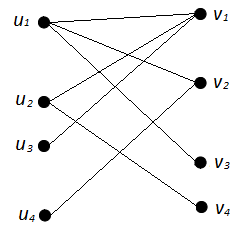
\includegraphics[width=50mm]{MatchingGraph}
	\caption{The matching graph $G(H)$ for the input trees in figure \ref{Fig:InputTrees}.}
	\label{matchingGraphFigure}
\end{figure}

A matching graph $G(x)$ is used to create a Largest Weight Agreement Matching which can be translated directly to the MAST of $T_1$ and $T_2(x)$. For each $u_i \in L(x)$, starting from the bottom, we compute the LWAM containing only edges from $u_i$ and nodes below $u_i$ in $L(x)$. This will be covered in detail in section \ref{agreementMatchingSection}.

\subsection{Creating the Matching Graphs}
First of all, a graph is created for each centroid path in $T_2$, where all nodes in the path is added to the right set. In order to get access to such a graph in constant time from a node in the path, we will make each start node of the paths point to the corresponding graph. Recall that each node of a path points to the start node.

Since the left set of each graph only contains nodes from $\pi$ we can add these nodes and all edges by doing a walk through $\pi$. This walkthrough contains the following steps for each node $z \in S_i$ for each $u_i \in \pi, 1 \le i \le p-1$, where the nodes of $S_i$ are traversed in preorder.

\begin{enumerate}
	\item Find the corresponding node $z'$ in $T_2$.
	\subitem This takes constant time since $z$ has a reference to $z'$.
	\item If $z'$ is on a centroid path $\pi(z')$ (this is the case if $z'$ has a pointer to the start node of a path), do the following:
	\subitem Find the graph $G(z')$ that corresponds to the path $\pi(z')$. This is done in constant time since $z'$ has a pointer to the start node $start(\pi(z'))$ which has a pointer to the graph.
	\subitem Add $u_i$ to $L(z')$ if it has not already been added.
	\subitem Add an edge between $u_i$ and $z'$ in $G(z')$.
	\subitem Repeat from step 2 using the parent of $start(\pi(z'))$ as node $z'$.
	\item If $z'$ is not on a centroid path, repeat from step 2 using the parent of $z'$.
\end{enumerate}
The loop stops either when reaching the root of $T_2$ or when reaching a node which is on the same path as the node in $T_2$ that corresponds to the parent of $z$ in $S_i$. The second case means that the rest of the processing has already been done by the parent. This ensures that for each node visited in $T_2$, an edge is added to some graph, meaning that the process of adding all edges takes linear time with respect to the total number of edges in the graphs. In the article \cite{nlogn}, an analysis proves that the total number of edges is bound by the sizes of the side trees of $\pi$ namely $O(\sum_{i=1}^{p-1}m_ilog\dfrac{n}{m_i})$ which is bound by $O(nlogn)$ since $\sum_{i=1}^{p} m_i = n$.

For the last node $u_p$ in $\pi$, the process is very similar. $z'$ starts being the twin of $u_p$ and the loop continues until reaching the root of $T_2$.\\

For any node $z \in S_i, 1 \le i \le p-1$, $z'$ being the corresponding node in $T_2$, every node $v_j$ visited in the iteration will be the node that is the closest ancestor of $z'$ in the path that $v_j$ is on, which means that either $z' \in N_j$ or $z'=v_j$. Both cases mean that $S_i \cap N_j \ne \emptyset$ so an edge should be added.

For $u_p$, $z'$ being the twin of $u_p$, if node $v_j$ is visited in the iteration, then $z' \in N_j$ so an edge should be added.

\subsection{Edge Weights}
Each edge in a graph is a multiedge consisting of a white, green and red edge, each with its own weight. The weights are defined as follows:
\begin{itemize}
	\item White edge weight: $weight_w(u_i, v_j)=$ size of $MAST(M_i,N_j)$
	\item Green edge weight: $weight_g(u_i, v_j)=$ size of $MAST(M_i,T_2(v_j))$
	\item Red edge weight: $weight_r(u_i, v_j)=$ size of $MAST(T_1(u_i),N_j)$
\end{itemize}

Let's again consider the input trees of figure \ref{Fig:InputTrees}. The edges of the matching graph $G(H)$ in figure \ref{matchingGraphFigure} are all multiedges that should get weights assigned to them. For example, the weight of the white edge $(u_1, v_1)$ is 2, since $MAST(M_1,N_1)$ is the tree having only the two leaves named $4$ and $6$. The weight of the green edge $(u_1, v_1)$ is 4, since $MAST(M_1,T_2(v_1))$ contains all four leaves of $M_1$.

The thing to notice about the edge weights is first that the size of a MAST is equal to the weight of the corresponding LWAM, and second that $LWAM(M_i, T_2) = LWAM(M_i, S_i), 1 \le i \le p-1$ which have already been computed in the recursive calls, so each node $v$ of $S_i$ holds the LWAM and its weight for $M_i$ and $S_i(v)$.

In order to compute the weight of each edge in constant time, a node $map(i,j)$ is defined for the multiedge $(u_i,v_j)$. $map(i,j)$ is the node of $S_i$ which is closest to the root and its corresponding node in $T_2$ is either a descendant of or equal to $v_j$. The edge $(u_i,v_j)$ is added to a graph during an iteration of a node in $S_i$, as described in the previous section. That node is exactly the node closest to the root in $S_i$ which is also a descendant or equal to $v_j$ in $T_2$, so a reference to $map(i,j)$ is added in constant time and doesn't change the time complexity.

First, if one of $u_i$ and $v_j$ is a leaf, then the weight of all three edges is 1. Otherwise, let $y=map(i,j)$.

\subsubsection{White Edge Weight}
$y$ is either a descendant of or equal to $v_j$. In the former case, we know that $y \in N_j$ or the edge would not have been added. So the weight of the white edge is the weight of $LWAM(M_i, S_i(y))$, which can be looked up at $y$ in constant time. In the latter case, one of $y's$ children is in $N_j$. That child $z$ is then the node closest to the root of $S_i$ which is in $N_j$, so the weight is equal to the weight of $LWAM(M_i, S_i(z))$, which is looked up in $z$. Since all nodes on a path of $T_2$ has a reference to the start node of that path, $z$ can be found in constant time by picking the child of $v_j$ that does not have a reference to the same node as $v_j$, i.e. it must be the root of $N_j$. If that node is the first child of $v_j$, then $z$ is the first child of $y$ and vice versa.

\subsubsection{Green Edge Weight}
The green edge weight is equal to the weight of $LWAM(M_i,T_2(v_j))$. $S_i(y)$ is the subtree of $T_2(v_j)$ containing only leaves of $M_i$, so the weight is equal to the weight of $LWAM(M_i, S_i(y))$ which is looked up at $y$ in constant time.

\subsubsection{Red Edge Weight}
Now let $y$ be the root of $N_j$, which we showed how to find in constant time. Since $y$ is a descendant of $x$ and the graphs and LWAMs are computed in order bottom the top, the LWAMs of $G(y)$, has already been computed. In that computation, the LWAM containing only edges from $u_i$ and nodes below $u_i$ in $L(y)$ was also computed, corresponding to $LWAM(T_1(u_i), N_j)$. The red edge weight is the weight of that matching which is looked up in constant time. We know that $u_i$ is in $L(y)$ since $M_i$ and $N_j = T_2(y)$ intersects.\\


The weight of each edge is computed in constant time, so the time of computing all edge weights is linear w.r.t. the number of edges which we showed is limited by $O(nlogn)$.

\section{Agreement Matchings}
\label{agreementMatchingSection}
An agreement matching is a subset of a matching graph $G(x), x \in X$, that corresponds to an agreement subtree between some subtree of $T_1$ and some subtree of $T_2(x)$.

For each $u_i \in L(x)$, starting from the bottom, we will compute the largest weight agreement matching containing only edges from $u_i$ and nodes below $u_i$ in $L(x)$ and for each $v_j \in R(x)$, we will compute the largest weight agreement matching containing only edges from $v_j$ and nodes below $v_j$ in $R(x)$.

This will be done for all matching graphs in order bottom to top, where a graph $G(x)$ is above the graph $G(x')$ if and only if $x$ is an ancestor of $x'$ in $T_2$. This means that the final LWAMs to be computed are from the matching graph $G(r)$, where $r$ is the root of $T_2$. The LWAM for $T_1$ and $T_2$ is then LWAM containing only edges from $u_1$ and nodes below $u_1$ in $L(r)$.

\subsection{Definitions}
We will start by describing some definitions used in agreement matchings.

\subsubsection{Nodes and Edges}
For nodes and edges in the graph $G(x)$ we have the following definitions:
\begin{itemize}
	\item $d_x(u_i)$: The 'degree' of a node $u_i \in L(x)$ is the number of white edges incident on it.
	\subitem A node in $L(x)$ is a 'singleton' node if it has degree 1.
	\subitem Edges incident on singleton nodes are called 'singleton' edges.
	\item $nsav(x)$: The number of nodes in $R(x)$ having at least one incident non-singleton edge.
\end{itemize}

For any edge $(u_i, v_j)$, we say that $u_i$ and $v_j$ are adjacent. For two edges $(a,b)$ and $(a',b')$ in $G(x)$, we will say they 'cross' if $a$ is above $a'$ in $L(x)$ and $b$ is below $b'$ in $R(x)$. The two edges 'touch' if they are either crossing or $a=a'$ or $b=b'$. Finally $(a,b)$ 'dominates' $(a',b')$ if $a$ is above $a'$ and $b$ is above $b'$.

\subsubsection{Agreement Matchings}
In the graph $G(x)$, a 'Proper Crossing' is either a single red edge, a single green edge or a crossing of a red edge $(u_i,v_j)$ and a green edge $(u_i',v_j')$ where $u_i'$ is above $u_i$ in $L(x)$.

Now an agreement matching is defined as a proper crossing and zero or more white edges, where all white edges dominate the edge(s) in the proper crossing and no white edge touches any other edge in the agreement matching.

This definition makes sure that an agreement matching holds exactly the information needed to uniquely determine the corresponding agreement subtree.

Consider again the matching graph from figure \ref{matchingGraphFigure}. Given this graph, an agreement matching could be the one in figure \ref{agreementMatchingFigure}, where the edge $(u_1,v_1)$ is white, the edge $(u_2,v_4)$ is green and the edge $(u_4,v_2)$ is red.

\begin{figure}
	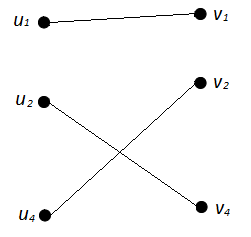
\includegraphics[width=50mm]{AgreementMatching}
	\caption{Example of an agreement matching.}
	\label{agreementMatchingFigure}
\end{figure}

\subsection{Agreement Matchings and MASTs}
Consider the two trees $T_1$ and $T_2$ giving the graph $G(x)$ for the topmost node $x$ in a centroid path $\pi(x)$ of $T_2$. $T_1$ has the centroid path $\pi$. For each multiedge $e = (u_i, v_j), u_i \in L(x), v_j \in R(x)$ of $G(x)$, the white edge of $e$ corresponds to the tree $MAST(M_i, N_j)$, the green edge of $e$ corresponds to $MAST(M_i, T_2(v_j))$ and the red edge of $e$ corresponds to $MAST(T_1(u_i), N_j)$. Since the weight of each edge in $G(x)$ is the size of its corresponding tree, the largest weight agreement matching gives the set of trees, satisfying the conditions for an agreement matching, with the maximum number of leaves. These trees will be side trees on a path in the MAST between $T_1$ and $T_2(x)$.

Consider the MAST $\mathcal{A}$ between $T_1$ and $T_2(x)$. Each node of $\mathcal{A}$ will correspond to both a node in $T_1$ and a node in $T_2(x)$. If $\mathcal{A}$ doesn't contain any node corresponding to a node from $\pi(x)$, then it must be equal to the MAST between $T_1$ and $N_j$ for some sidetree $N_j$ of $\pi(x)$. If $u_i$ is the topmost node in $\pi$ for which $M_i \cap N_j \ne \emptyset$, then $MAST(T_1, N_j) = MAST(T_1(u_i), N_j)$ which can be represented by a single red edge between $u_i$ and $v_j$. If $\mathcal{A}$ doesn't contain any node corresponding to a node from $\pi$, it is equal to the MAST between $M_i$ and $T_2(x)$ for some sidetree $M_i$ of $\pi$. If $v_j$ is the topmost node in $\pi(x)$ for which $M_i \cap N_j \ne \emptyset$, then $MAST(M_i, T_2(x)) = MAST(M_i, T_2(v_j))$. This MAST would be represented by a single green edge between $u_i$ and $v_j$.

Now let's look at the final case where $\mathcal{A}$ contains nodes from both $\pi$ and $\pi(x)$. Then at least one node in $\mathcal{A}$ will correspond to both a node in $\pi$ and a node in $\pi(x)$. This will always be the case for the root of $\mathcal{A}$. Let $w$ be one such node and $u_i \in \pi$ and $v_j \in \pi(x)$ be the nodes in $T_1$ and $T_2$ corresponding to $w$.

If $w$ is not the bottommost such node in $\mathcal{A}$, then one of its children is too, and the other is not. Let $z$ be the child which is not. Then $\mathcal{A}(z)$ must be the MAST between $M_i$ and $N_j$. This MAST can be represented by a single white edge between $u_i$ and $v_j$.

Now assume that $w$ is indeed the bottommost such node in $\mathcal{A}$. If $w$ is a leaf, then $u_i$ is the leaf $u_p$ and $v_j$ is the leaf $v_q$ and $\mathcal{A}$ is the MAST between $T_1(u_p)$ and $N_q$ which is represented by a single red edge between $u_p$ and $v_q$. If $w$ is not a leaf, then the subtrees rooted at the two children of $w$ are one of the following.

\begin{itemize}
	\item One subtree is the MAST between $M_i$ and $N_j$. The other is the MAST between $T_1(u_{i+1})$ and $N_j'$ for some $j', j < j' \le q$.
	\item One subtree is the MAST between $M_i$ and $N_j$. The other is the MAST between $M_i'$ and $T_2(v_{j+1})$ for some $i', i < i' \le p$.
	\item One subtree is the MAST between $T_1(u_{i+1})$ and $N_j$. The other is the MAST between $M_i$ and $T_2(v_{j+1})$.
\end{itemize}

The first case can be represented by a white edge between $u_i$ and $v_j$ and a red edge between $u_{i'}$ and $v_{j'}$, where $u_{i'}, i' > i$ is the topmost node below $u_i$ in $\pi$ for which $M_{i'} \cap N_{j'} \ne \emptyset$.

The second case can be represented by a white edge between $u_i$ and $v_j$ and a green edge between $u_{i'}$ and $v_{j'}$, where $v_{j'}, j' > j$ is the topmost node below $v_j$ in $\pi(x)$ for which $M_{i'} \cap N_{j'} \ne \emptyset$.

The third case can be represented by a red edge between $u_{i'}$ and $v_{j}$, where $u_{i'}, i' > i$ is the topmost node below $u_i$ in $\pi$ for which $M_{i'} \cap N_{j} \ne \emptyset$ and a green edge between $u_{i}$ and $v_{j'}$, where $v_{j'}, j' > j$ is the topmost node below $v_j$ in $\pi(x)$ for which $M_{i} \cap N_{j'} \ne \emptyset$.\\

All possible cases of $\mathcal{A}$ has been covered and in each case the the subtrees of $\mathcal{A}$ could be represented by edges in an agreement matching.

\subsection{The Weighted Search Tree}
In order to compute the LWAMs in $O(nlogn)$ time, we will create a weight balanced binary search tree $\mathcal{T}$ for each matching graph $G(x)$. This tree will be used to store the information needed to determine which edges of $G(x)$ forms the LWAMs. The structure of the tree will ensure that filling the tree and extracting the LWAMs will not take more than $O(nlogn)$ time.

$\mathcal{T}$ is created from the nodes in $R(x)$ such that $\mathcal{T}$ will have a leaf for each node in $R(x)$. The order of the leaves from left to right should correspond to the top-down order of the nodes in $R(x)$ such that the leftmost leaf in $\mathcal{T}$ corresponds to the topmost node in $R(x)$. Leaf $v_j$ is given weight $n_j + \frac{|T_2(x)|}{nsav(x)}$ if a non-singleton edge in $G(x)$ has endpoint in $v_j$ and weight $n_j$ otherwise. The reason for choosing these weights is explained later.

Recall that for each $u_i \in L(x)$, we want to compute the LWAM containing only edges from $u_i$ and nodes below $u_i$ in $L(x)$. This is done by processing each node $u_i \in L(x)$ in order bottom-to-top, where each node in $R(x)$, that has an edge to $u_i$, is searched for in $\mathcal{T}$, while storing information about the edges in $\mathcal{T}$.  After processing $u_i$, the LWAM can be extracted from $\mathcal{T}$. 

\subsubsection{Constructing the Weighted Search Tree}
For a matching graph $G(x)$, the weighted search tree can be constructed in $O(|R(x)|)$ time. Since $\sum_{x \in X} |R(x)| = n$, all the search trees needed for the matching graphs can be constructed in $O(n)$ time. This is not covered by Cole et. al. \cite{nlogn}, but in the paper \cite{fredman} by Fredman, it it described how a balanced search tree can be constructed in $O(N)$ time, given $O(N)$ probabilities which should be associated with the nodes of the tree.

Though not completely applicable to our situation, we used it as a basis for the following algorithm. Each node in the tree will get an index number which is used for searching.

\begin{itemize}
	\item Given weights ${w_0, w_1, ..., w_{|R(x)|-1}}$, construct two lists of sums ${L_0, ..., L_{|R(x)|}}$ and ${R_0, ..., R_{|R(x)|}}$, where
	\subitem $L_j=\sum_{k=0}^{j-1} w_k$, $L_0=0$
	\subitem $R_j=\sum_{k=j}^{|R(x)|-1} w_k$, $R_{|R(x)|}=0$
	\item Construct the tree using the recursive procedure $constructST(w_0, w_1, ..., w_{|R(x)|-1})$ which returns the root of the search tree.
	\item $constructST(w_i, ..., w_j)$ has the following steps:
	\subitem If $i+1=j$ then create and return a node with index $j$ having a left child with index i and a right child with index j.
	\subitem Otherwise, determine the smallest $k, i<k\le j$ such that
	\subsubitem $L_k-L_i \ge R_k-R_{j+1}$
	\subitem Define a node with index $k$ having $constructST(w_i, ..., w_{k-1})$ as left child and $constructST(w_k, ..., w_j)$ as right child.
	\subsubitem If $i=k-1$, the left child is just a leaf with index $i$.
	\subsubitem If $k=j$, the right child is just a leaf with index $j$.
\end{itemize}

Determining $k$ from the weights ${w_i, ..., w_j}$ is done by finding the smallest $k$ satisfying $L_k-L_i \ge R_k-R_{j+1}$. This can be done in $O(log(k-i))$ time as follows:

\begin{itemize}
	\item For the middle index $k'=i+(j-i+1)/2$, determine whether $L_{k'}-L_i \ge R_{k'}-R_{j+1}$.
	\item If so, let $k'=i+1, k'=i+2, k'=i+4, k'=i+8, ...$ until $L_{k'}-L_i \ge R_{k'}-R_{j+1}$.
	\subsubitem This takes $O(log(k'-i))$ time for the final value of $k'$.
	\subsubitem $k'-i \le 2(k-i)$, so $O(log(k'-i)) = O(log(k-i))$.
	\subitem In the interval between $k'$ and the previous value of $k'$, use binary search to find the smallest $k'$ satisfying $L_{k'}-L_i \ge R_{k'}-R_{j+1}$.
	\subsubitem This takes $O(log(k-i))$ time.
	\subitem Then $k=k'$.
	\item The case where $L_{k'}-L_i < R_{k'}-R_{j+1}$ is treated symmetrically.\\
\end{itemize}
The linear time complexity can be explained as follows:

Let $F(N)$ be the time taken to construct a search tree with $N$ internal nodes. $F(N)$ satisfies the following inequality

$F(N) \le max\{A + Blog(k) + F(k-1) + F(N-k), 1 \le k \le (N+1)/2\}$

where $A$ and $B$ are constants and $N$ and $k$ are natural numbers. This function can be proven to grow at most linearly with $N$, thus constructing a search tree has linear runtime w.r.t. the number of internal nodes. The proof can be seen in section \ref{searchTreeProof}. $|R(x)|$ is greater than the number of internal nodes, so a weight balanced binary search tree can be constructed in $O(|R(x)|)$ time.

\subsubsection{Searching}
\label{st_searching}
In order to minimize the runtime when searching for leaves in the search tree $\mathcal{T}$, we will specify how two kinds of searches should be performed.

In a search tree $\mathcal{T}$, each node $v$ will hold an index number $index(v)$. Searching for a leaf in $\mathcal{T}$ with index number $i$, is done in the standard way by starting at the root and picking the left child if $i < the$ $current$ $node$ $index$, and the right child otherwise until reaching the desired leaf.

Each node $v$ will also hold the lowest index number $low(v)$ and largest index number $high(v)$ in its subtree, which is used when searching for an ordered subset of $R(x)$. These numbers are added while creating the tree. For the root $r$, $low(r)$ is 0 and $high(r)$ is $|R(x)|-1$. For a left child $v$, $low(v)=low(parent(v))$ and $high(v)=index(parent(v))-1$. For a right child $v$, $low(v)=index(parent(v))$ and $high(v)=high(parent(v))$.

Given the subset ${v_i, ..., v_j}$ of $R(x)$ in bottom to top order, let ${l_i, ..., l_j}$ be the corresponding leaves in $\mathcal{T}$. Searching for these leaves is done with a sequential search by first searching for the leaf $l_i$ in the standard way. When at a leaf $l_{i'}, i' < j$, searching for $l_{i'+1}$ is done by starting at $l_{i'}$ and go up through the tree until reaching a node whose lowest index number is less than or equal to $index(l_{i'+1})$. $l_{i'+1}$ is now found by searching in the standard way starting at the node just reached.

Given a subset of $R(x)$ in top to bottom order, searching for the corresponding leaves in $\mathcal{T}$ is done similarly, but considering the largest index numbers instead of the lowest.

\subsubsection{Properties of the Search Tree}
\label{stProperties}
A search tree $\mathcal{T}$ is created such that a leaf $l$ corresponding to $v_j \in R(x)$ has weight $n_j + \frac{|T_2(x)|}{nsav(x)}$ if a non-singleton edge in $G(x)$ has endpoint in $v_j$ and weight $n_j$ otherwise. Balancing the tree with these weights ensures that the depth of any leaf $l$ corresponding to node $v_j \in R(x)$ is $O(log\frac{|T_2(x)|}{n_j})$. When searching for an ordered subset of $k$ leaves in $\mathcal{T}$ as specified in the previous section, the structure of $\mathcal{T}$ also ensures that the number of nodes visited is $O(k*log \dfrac{nsav(x)}{k})$ and each node is visited a most thrice. The reasoning behind these claims can be found in \cite{nlogn}.

\subsection{Computing the Largest Weight Agreement Matchings}
Computing the LWAM for the graph $G(x)$ is done by processing each node of $L(x)$ in order starting with the bottom node. Recall that we will compute the LWAM containing only edges from $u_i$ and nodes below $u_i$ in $L(x)$, for each $u_i \in L(x)$. This is done by adding that information to $\mathcal{T}$ while processing the nodes of $L(x)$. 

First, we will describe the information that needs to be stored in $\mathcal{T}$. Next, we will explain how nodes are processed and show how to process each colour edge and afterwards explain the order that the edges need to be processed in. Then we will show how to extract the LWAMs from $\mathcal{T}$ and finally explain the total time complexity of this step.

\subsubsection{Auxiliary Information in $\mathcal{T}$}
While processing the edges of $G(x)$ we will maintain information at each node of $\mathcal{T}$ about the LWAM of the currently processed edges. For a node $z \in \mathcal{T}$, we define $anc(z)$ as the set of ancestors of $z$, including $z$ itself in order top to bottom. $lfringe(z)$ is defined as the left children of the vertices in $anc(z)$ which are not in $anc(z)$ themselves. $lfringe$ will only contain nodes with indices less than $index(z)$. $rfringe(z)$ is defined analogously where the nodes all have indices greater or equal to $index(z)$. $anc(z)$ need not be stored in $\mathcal{T}$, but can be created while searching for $z$ in $\mathcal{T}$. Likewise, $lfringe(z)$ and $rfringe(z)$ can be created by iterating through $anc(z)$. After processing an edge $(u,v)$, we say that the edge is in $\mathcal{T}$. For a node $z \in \mathcal{T}$ we also say that $(u,v)$ is in $T(z)$ if $T(z)$ contains the node corresponding to $v$.

The following information is maintained at each node $z \in \mathcal{T}$. This is taken directly from \cite{nlogn}, but slightly elaborated.
\begin{itemize}
	\item $g(z)$: After updating $g(z)$, it will hold the heaviest green edge in $\mathcal{T}$ which	forms a proper crossing with each red edge in $\mathcal{T}(z)$.
	\subitem However, $g(z)$ is not maintained at all times, but the correct edge can be retrieved from $max_{z' \in anc(z)}g(z')$.
	\subitem If there are no red edges in $\mathcal{T}(z)$ when updating $g(z)$, then $g(z)$ will be the heaviest green edge in $\mathcal{T}(z')$, for all $z' \in rfringe(z)$.
	\item $x(z)$: This is the largest weight proper crossing, that is not a single red edge, among the edges in $\mathcal{T}(z)$.
	\item $m(z)$: This is the largest weight agreement matching containing a white edge
	such that the topmost white edge is in $\mathcal{T}(z)$.
	\item $y(z)$: This the largest weight proper crossing, which is not a single edge, such that the green edge is in $\mathcal{T}$ but not in $\mathcal{T}(z)$, the red edge is in $\mathcal{T}(z)$, and the green edge does not form a proper crossing with all the red edges in $\mathcal{T}(z)$.
	\item $r(z)$: This is simply the heaviest red edge in $\mathcal{T}(z)$.
\end{itemize}

\subsubsection{Processing Nodes}
For each node $u_i \in L(x)$, starting from the bottommost, we need to process each edge $e = (u_i, v_j)$ incident on it. This is done by searching for the leaf corresponding to $v_j$ in $\mathcal{T}$ and updating information at nodes in $\mathcal{T}$ so that $e$ is contained in $\mathcal{T}$. Leaves are searched for as described in section \ref{st_searching}, where a standard search is used if $d_x(u_i) = 1$ and a sequential search is used if $d_x(u_i) > 1$.

In the following, we will explain how each colour edge is processed when $d_x(u_i) = 1$ and afterwards when $d_x(u_i) > 1$. Let $e=(u_i,v_j)$ be the edge in $G(x)$ that should be processed and $l$ be the leaf in $\mathcal{T}$ corresponding to $v_j$. We know that all edges incident on nodes below $u_i$ in $L(x)$ have already been processed.

\subsubsection{Processing singleton white edges}
The only values that might change in $\mathcal{T}$ when adding a white edge is $m(z), z \in anc(l)$. First, $anc(l)$ is found while searching for $l$ in $\mathcal{T}$ and $rfringe(l)$ is subsequently created. Now the LWAM with $e$ as topmost edge needs to be determined. This is done by finding the LWAM containing only edges dominated by $e$ and then adding $e$ as the topmost white edge. Since the nodes of $L(x)$ are processed starting from the bottom, we know that $\mathcal{T}$ does not contain any edges incident on nodes above $u_i$ in $L(x)$. The subtrees of nodes in $rfringe(l)$ contain exactly the edges in $\mathcal{T}$ only incident on nodes below $v_j$ in $R(x)$. %By the order we process the edges, we also make sure that the edges from $u_i$ are processed such that $rfringe(l)$ contains no edge incident on $u_i$.
There are four cases of LWAMs:
\begin{itemize}
	\item The LWAM contains one or more white edges.
	\subitem This matching is given by $max_{z \in rfringe(l)} m(z)$
	\item The LWAM is a single green edge or a green-red crossing where both edges are in the subtree $\mathcal{T}(z)$ for some $z \in rfringe(l)$.
	\subitem This matching is given by $max_{z \in rfringe(l)} x(z)$
	\item The LWAM is a single red edge or a green-red crossing where the red edge is in the subtree $\mathcal{T}(z)$ for some $z \in rfringe(l)$. The green edge forms a proper crossing with all red edges in $\mathcal{T}(z)$.
	\subitem This matching is given by $max_{z \in rfringe(l)} (max_{z' \in anc(z)} g(z')) + r(z)$
	\item The LWAM is a green-red crossing where the red edge is in the subtree $\mathcal{T}(z)$ for some $z \in rfringe(l)$. The green edge is not in $\mathcal{T}(z)$ and does not form a proper crossing with all red edges in $\mathcal{T}(z)$.
	This matching is given by $max_{z \in rfringe(l)} y(z)$
\end{itemize}

These cases cover all possible LWAMs containing only edges dominated by $e$, so adding $e$ as the topmost white edge to the largest of these agreement matchings, gives us the LWAM that should replace $m(z), z \in anc(l)$ if it has larger weight than the agreement matching already stored.

In order to avoid copying the agreement matching just found, which would take linear time w.r.t. the number of edges, the new agreement matching can be stored as the white edge $e$ and a pointer to the other agreement matching. This will also minimize the amount of space needed.

\subsubsection{Processing singleton red edges}
The values that might change in $\mathcal{T}$ when adding a red edge is $y(z), g(z)$ and $r(z), z \in anc(l)$ and $g(z'), z' \in lfringe(l) \cup rfringe(l)$. Since none of the green edges in $\mathcal{T}$ can form a proper crossing with $e$, $y(z)$ might change for $z \in anc(l)$. So $y(z)$ is updated to $max\{y(z), (max_{z' \in anc(z)} g(z')) + r(z)\}$. Now $g(z)$ should be reset for all $z \in anc(l)$. However, in order to maintain all $g$ values in $\mathcal{T}$, $g(z')$ needs to be updated to $max_{z'' \in anc(z')} g(z'')$ for each $z' \in lfringe(l) \cup rfringe(l)$ before resetting. Finally, $r(z)$ need to be updated for $z \in anc(l)$ if the weight of $e$ is greater than that the current value of $r(z)$. $r(z)=max\{r(z), e\}$.

\subsubsection{Processing singleton green edges}
Adding a green edge to $\mathcal{T}$ might change the values $g(z), z \in lfringe(l)$ and $x(z), z \in anc(l)$. When adding the green edge $e$, it will form proper crossings with all red edges in $\mathcal{T}$ incident on nodes in $R(x)$ above $v_j$. This is true since each red edge in $\mathcal{T}$ is incident on a node in $L(x)$ below $u_i$. Therefore $g(z), z \in lfringe(l)$ is updated to $e$ if the weight of $e$ is greater than that of the currently heaviest green edge forming a proper crossing with all red edges in $\mathcal{T}(z)$. $g(z)=max\{e, max_{z' \in anc(z)} g(z')\}, z \in lfringe(l)$. The value $x(z), z \in anc(l)$ might also need to be updated if the proper crossing between $e$ and a red edge in $\mathcal{T}(z)$ is heavier than the current value of $x(z)$. $x(z)=max\{x(z), e + max(r(z'))\}, z \in anc(l)$. Here $max(r(z'))$ maximizes over the vertices $z' \in lfringe(l)$ which are descendants of $z$.

\subsubsection{Processing nodes with degree > 1}
Recall that we process the edges by iterating through $L(x)$ starting from the bottommost node, and process the edges incident on each of these nodes. For a node $u_i \in L(x)$ we will start by processing the white edges incident on $u_i$ in order, starting from the topmost edge, i.e. the edge incident on the topmost node in $R(x)$. The reason for doing top-down processing is explained later. For these edges, the leaves in $\mathcal{T}$ that needs to be searched for, are found with a sequential search as described in section \ref{st_searching}.

Next, we process the red and green edges incident on $u_i$ in order, starting from the bottommost edge. This ensures that when processing a green edge $e=(u_i,v_j)$, no red edges incident on $u_i$ and on a node in $R(x)$ above $v_j$ has been processed. Searching for leaves in $\mathcal{T}$ is also done with sequential search.

Processing edges from non-singleton nodes using sequential search is crucial for the runtime of this step. Let ${l_1, l_2, ..., l_k}$ be the leaves in the search tree that are searched for when processing $u_i \in L(x)$. The only nodes in the search tree that need to be updated are nodes from the set ${anc(l_1) \cup anc(l_2) \cup ... \cup anc(l_k)}$, but in order to ensure that only a constant amount of work is performed at each node, we need a slightly different approach than for the singleton edges. This was not covered by Cole et. al. \cite{nlogn}, so we came up with our own approach.

In the following, we will explain how each colour edge is processed when $d_x(u_i) > 1$. Let $e_1, e_2, ...$ be the edges in $G(x)$ incident on $u_i$ and $l_1, l_2, ...$ be the corresponding leaves in $\mathcal{T}$ that should be searched for. The white edges are in top-down order and the red and green edges are in bottom-up order. Again, we know that all edges incident on nodes below $u_i$ in $L(x)$ have already been processed.

\subsubsection{Processing white non-singleton edges}
For processing white non-singleton edges, we will introduce some extra information that should be stored in $\mathcal{T}$, but only while processing the white edges incident on $u_i$.

The following information is stored at each node $z \in {anc(l_1) \cup anc(l_2) \cup ... }$ as they are being visited the first time.

\begin{itemize}
	\item $rm(z)$: This is the heaviest of the agreement matching of $m(z'), z' \in rfringe(z)$.
		\subitem $rm(z) = max_{z'\in rfringe(z)} m(z')$
	\item $rx(z)$: This is the heaviest of the agreement matching of $x(z'), z' \in rfringe(z)$.
		\subitem $rx(z) = max_{z'\in rfringe(z)} x(z')$
	\item $ry(z)$: This is the heaviest of the agreement matching of $y(z'), z' \in rfringe(z)$.
		\subitem $ry(z) = max_{z'\in rfringe(z)} y(z')$
	\item $ag(z)$: This is the heaviest of the edges $g(z'), z' \in anc(z)$.
		\subitem $ag(z) = max_{z'\in anc(z)} g(z')$
	\item $gr(z)$: This is the heaviest single red edge or green-red proper crossing where the red edge is in the subtree $\mathcal{T}(z')$ for some $z' \in rfringe(z)$. The green edge forms a proper crossing with all red edges in $\mathcal{T}(z')$.
		\subitem $gr(z) = max_{z'\in rfringe(z)} (max_{z''\in anc(z')} g(z'')) + r(z')$
\end{itemize}

Searching for leaves in $\mathcal{T}$ is done by starting from the root of $\mathcal{T}$. Thus finding the above values can be done in constant time for each node $z$ in the following way, where $p(z)$ is the parent node of $z$:
\begin{itemize}
	\item $ag(z) = max\{ag(p(z)), g(z)\}$
	\item If $z$ is the left child of its parent $p(z)$ and $z'$ is the right child, then
		\subitem $rm(z) = max\{rm(p(z)), m(z')\}$
		\subitem $rx(z) = max\{rx(p(z)), x(z')\}$
		\subitem $ry(z) = max\{ry(p(z)), y(z')\}$
		\subitem $gr(z) = max\{gr(p(z)), ag(z') + r(z')\}$
	\item Otherwise if $z$ is the right child of its parent $p(z)$, then
	\subitem $rm(z) = rm(p(z))$
	\subitem $rx(z) = rx(p(z))$
	\subitem $ry(z) = ry(p(z))$
	\subitem $gr(z) = gr(p(z))$
\end{itemize}

Processing the white edges in top-down order ensures that when processing a white edge $e_{j'}=(u_i,v_j)$, no other edge incident on $u_i$ and on a node in $R(x)$ below $v_j$ has been processed. This means that the agreement matchings $rm(l_{j'}), rx(l_{j'}), ry(l_{j'})$ and $gr(l_{j'})$ only contains edges dominated by $e_{j'}$.

When processing the topmost edge $e_1$, we will search for leaf $l_1$ in $\mathcal{T}$ with a standard search while storing the above values at the nodes of $anc(l_1)$. Now as when processing singleton white edges, we need to find the LWAMs containing only edges dominated by $e_1$ and then adding $e_1$ as the topmost white edge. These LWAMs are exactly the ones we have now stored at $l_1$: $rm(l_1), rx(l_1), ry(l_1)$ and $gr(l_1)$. The largest weight agreement matching with $e_1$ as topmost white edge is therefore the heaviest of these agreement matchings with $e_1$ added as topmost white edge. Now the values $m(z), z \in anc(l_1)$ needs to be updated with this LWAM, but since the remaining edges incident on $u_i$ might have some of the same ancestors, we will instead update the values while searching for these edges.

When searching for a leaf $l_{j'}, j' > 1$, starting at $l_{j'-1}$, we first go up through the tree until reaching the first node which is an ancestor of both $l_{j'}$ and $l_{j'-1}$ and afterwards search for $l_{j'}$ in the standard way while updating values at the nodes visited as before. While going up through the tree, we can update the nodes visited with the LWAM found when processing the previous edge $e_{j'-1}$, since these nodes are all ancestors of $l_{j'-1}$. Reaching a node $z$ where $m(z)$ is heavier than the agreement matching we are currently updating with, means that it is an agreement matching found when processing one of the previous edges, so the following nodes should instead be updated with that matching.

Having processed the last edge, we will continue to the root of $\mathcal{T}$ in order to update the remaining ancestors.

\subsubsection{Processing red and green non-singleton edges} 
The only extra information that should be stored in $\mathcal{T}$ while processing red and green edges incident on $u_i$ is $ag(z)$ for each node $z \in {anc(l_1) \cup anc(l_2) \cup ... }$. $ag(z)$ is defined as when processing white non-singleton edges and found the same way while searching for leaves in $\mathcal{T}$.

The procedure is similar to processing white non-singleton edges. The leaves of $\mathcal{T}$ are searched for using sequential search, but starts from the bottommost edge. In the end, we return to the root of $\mathcal{T}$.
\\
\\
As when processing singleton edges, adding a red edge $e_{j'}$ to $\mathcal{T}$ might changes the values $y(z), g(z)$ and $r(z), z \in anc(l_{j'})$ and $g(z'), z' \in lfringe(l_{j'}) \cup rfringe(l_{j'})$. For $z \in anc(l_{j'})$, $y(z)$ should be updated to $max\{y(z), (max_{z' \in anc(z)} g(z')) + r(z)\} = max\{y(z), ag(z) + r(z)\}$. For each $z \in lfringe(l_{j'}) \cup rfringe(l_{j'})$, $g(z)$ should be updated to $max_{z' \in anc(z)} g(z') = ag(z)$ and for $z \in anc(l_{j'})$, $g(z)$ should be reset and $r(z)$ updated to $max\{r(z), e_{j'}\}$.

Having stored $ag(z)$ at each node $z$ visited while searching, all of the above values can be updated in constant time for each node while going up through the tree.

Notice that when resetting $g(z)$ for some node $z$, $ag(z)$ also needs to be reset since $z$ might be visited again and the value of $ag(z)$ is no longer valid.
\\
\\
Adding a green edge $e_{j'}$ to $\mathcal{T}$ might changes the values $g(z), z \in lfringe(l_{j'})$ and $x(z), z \in anc(l_{j'})$. For $z \in lfringe(l_{j'})$, $g(z)$ is updated to $max\{e_{j'}, max_{z' \in anc(z)} g(z')\} = max\{e_{j'}, ag(z)\}$. Since $ag(z)$ is stored at each node $z$ visited while searching, $g(z), z \in lfringe(l_{j'})$ is updated in constant time for each node while going up through the tree. For $z \in anc(l_{j'})$, $x(z)$ should be updated to $max\{x(z), e_{j'} + max(r(z'))\}$, where $max(r(z'))$ maximizes over the vertices $z' \in lfringe(l_{j'})$ which are descendants of $z$. This is also done in constant time for node $z \in anc(l_{j'})$ while going up through the tree by keeping track of the heaviest red edge $hre$ of $r(z'), z' \in lfringe(l_{j'})$, where $z'$ is a descendant of $z$.

If $z$ is the first node which is an ancestor of both $l_{j'}$ and $l_{j'+1}$ (assuming that $l_{j'+1}$ exists), we will store $e_{j'}$ at $z$ as $ge(z)$. Now when going up through the tree after having reached leaf $l_{j'}$, we will also keep track of which green edge $hge$, incident on $u_i$ is the heaviest that has been added to the subtree rooted at the current node $z$. When at $l_{j'}$, $hge$ is obviously $e_{j'}$, and when at a node $z \in anc(l_{j'})$ it is simply the heaviest edge of $hge$ and $ge(z)$. $x(z)$ can now be updated to $max\{x(z), hge + hre\}$.

\subsubsection{Extracting the Largest Weight Agreement Matchings}
First, we need to compute the LWAM containing only edges from $u_i$ and nodes below $u_i$ in $L(x)$, for each $u_i \in L(x)$. For any $u_i \in L(x)$, all the information needed to compute such a matching is stored at the root $r$ of $\mathcal{T}$ after having processed the edges incident on $u_i$ and before processing edges incident on the above nodes in $L(x)$. The LWAM is extracted in the following way:

If the LWAM contains a white edge it is simply given by $m(r)$. If the LWAM is a proper crossing, but not a single red edge, it is given by $x(r)$. And finally, if the LWAM is a single red edge, it is given by $r(r)$. Therefore the LWAM is the heaviest of these three matchings. This LWAM is saved, such that it can be retrieved in constant time given $u_i$ and $x$. 

For each $v_j \in R(x)$, we also need to compute the LWAM containing only edges incident on $v_j$ and nodes below $v_j$ in $R(x)$. For leaf $v_j \in R(x)$, such a matching will correspond to the MAST between $T_1$ and $T_2(v_j)$, so this is the LWAM that needs to be stored at $v_j \in T_2$. The LWAMs are extracted from $\mathcal{T}$, after all edges in $G(x)$ have been processed, in the following way:

For node $v_j \in R(x)$, let $l$ be the leaf in $\mathcal{T}$ corresponding to $v_j$ and let $M(v_j)$ be the LWAM containing only edges incident on $v_j$ and nodes below $v_j$ in $R(x)$. $M(v_j)$ is either equal to $M(v_{j+1}), j \ne |R(x)|$ (-1?), or it is the LWAM having a white edge incident on $v_j$ as the topmost edge, or it is the largest proper crossing having a red edge incident on $v_j$, or it is a single green edge incident on $v_j$. Thus, $M(v_j)$ is given by $max\{M(v_{j+1}), m(l), y(l), max_{z \in anc(l)}g(z) + r(l), x(l)\}$ where $M(v_{|R(x)|+1}) = 0$.

After having computed the LWAMs for all matching graphs, the LWAM corresponding to the MAST between $T_1$ and $T_2$ can be retrieved in constant time from the root $u_1$ of $T_1$ and the root $v_1$ of $T_2$. This was extracted from the search tree for the matching graph $G(v_j)$ and is the LWAM containing edges from $u_1$ and nodes below $u_1$ in $L(v_j)$ which is all possible edges and therefore corresponds to the MAST between $T_1$ and $T_2$.

\subsubsection{Analysis}
\label{lwam_analysis}
In \cite{nlogn}, Cole et. al. proves two important lemmas:

Lemma 4.1: Consider matching graph $G(x)$. Then

$\sum_{i|d_x(u_i)>1} d_x(u_i)log\dfrac{nsav(x)}{d_x(u_i)} \le \sum_{i|d_x(u_i)>1} d_x(u_i)log\dfrac{n}{m_i}$

Lemma 4.2: Consider node $u_i \in \pi$. Then

$\sum_{x \in X | d_x(u_i)>1} d_x(u_i) = O(m_i)$
\\
\\
Consider the matching graph $G(x)$ with search tree $\mathcal{T}$ and a node $u_i \in L(x)$. If $d_x(u_i) > 1$ and $L$ is the ordered set of leaves in $\mathcal{T}$ that corresponds to the nodes in $R(x)$ incident on the edges from $u_i$, then it follows from the claims in section \ref{stProperties} and Lemma 4.1 that the amount of nodes in the search tree that is visited when searching for the leaves of $L$ is $O(d_x(u_i)log(\dfrac{n}{m_i}))$.

Considering node $u_i \in \pi$, it follows from Lemma 4.2 that the amount of nodes visited in all search trees over all matching graphs $G(x)$ with $d_x(u_i) > 1$ is $O(m_ilog\dfrac{n}{m_i})$.

For each node $u_i \in \pi$ over all matching graphs $G(x)$ with $d_x(u_i) = 1$, it turns out that the amount of nodes visited in all search trees is also $O(m_ilog\dfrac{n}{m_i})$. This can be seen from the analysis in \cite{nlogn}.

Thus the total amount of nodes visited in all search trees, for any node $u_i \in \pi$, is $O(m_ilog\dfrac{n}{m_i})$.

\subsubsection{Time Complexity}
When searching for an ordered set of leaves in a search tree, each node is visited at most thrice and updating information in a search tree is done at the visited nodes and children of these nodes while searching. So for any node $u_i \in \pi$, the time taken to process $u_i$ over all matching graphs is $O(m_ilog\dfrac{n}{m_i})$.

Extracting the LWAM for edges from $u_i$ and nodes below $u_i$ in $L(x)$, for each $u_i \in L(x)$ takes constant time after having processed $u_i$. Extracting the LWAM for edges from $v_j$ and nodes below $v_j$ in $R(x)$, for each $v_j \in R(x)$ is done through a single traversal of $\mathcal{T}$ in $O(|R(x)|)$ time. This means that the total time for computing the largest weight agreement matchings is $O(\sum_{i=1}^p m_ilog\dfrac{n}{m_i}) \le O(nlogn)$.

\section{Creating the Maximum Agreement Subtree}
The last step of the algorithm is to construct the maximum agreement subtree from the LWAMs that have been computed.

As mentioned earlier, the Largest Weight Agreement Matching constructed from a matching graph $G(x)$ corresponds to the Maximum Agreement Subtree between $T_1$ and $T_2(x)$. We will show how the MAST $\mathcal{A}$ can be constructed given the LWAM with white edges ${we_1, we_2, ...}$ and proper crossing with edges ${ge, re}$ or single edge $ge$ or $re$ (See figure \ref{lwam_mast_figure}).

Recall that a white edge $(u_i, v_j)$ corresponds to the subtree $MAST(M_i,N_j)$, a green edge corresponds to $MAST(M_i,T_2(v_j))$ and a red edge corresponds to $MAST(T_1(u_i),N_j)$. These subtrees will appear in $\mathcal{A}$ in the same order that the edges appear in the matching. $\mathcal{A}$ will have an internal node for each white edge which forms a path ${p_1, p_2, ...}$ through $\mathcal{A}$. These nodes will be in the same order that the white edges appear in the matching. The off-path child of node $p_i$ will then be the root of the subtree corresponding to edge $we_i$. The second child $c$ of the last node in the path will hold the subtree(s) corresponding to the edge(s) in the proper crossing. If the proper crossing is a single edge, $c$ will be the root of the subtree corresponding to that edge. Otherwise $c$ will have two children, one being the root of the subtree corresponding to $ge$ and one being the root of the subtree corresponding to $re$.

\begin{figure}
	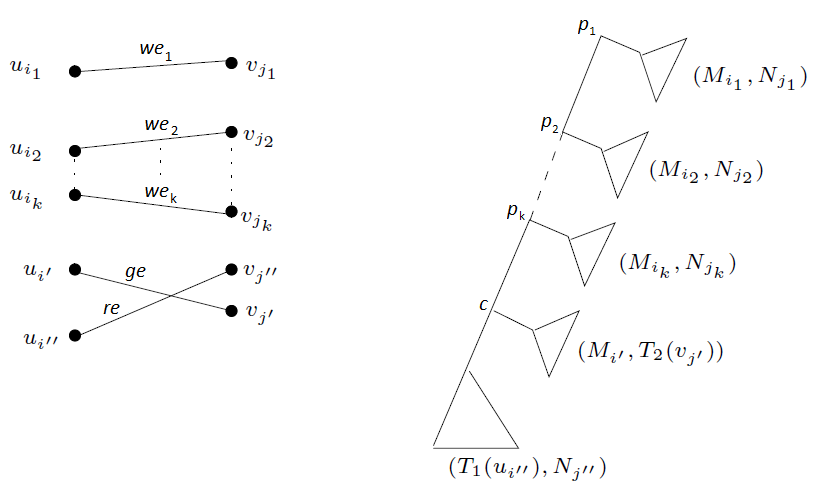
\includegraphics[width=\textwidth]{LWAMAndMAST}
	\caption{An Agreement Matching with the Associated Agreement Subtree. \cite{nlogn}}
	\label{lwam_mast_figure}
\end{figure}

What we need now is to find the subtrees corresponding to the edges in the matching. All the LWAMs corresponding to these subtrees have already been computed. Each is found in constant time by the same procedure as the edge weights were determined. \todo{explain?} \todo{store subtrees/matchings at edges??}. The subtrees can now be constructed recursively.

\subsection{Challenges} \todo{Maybe a whole section for challenges?}
Our first approach to construct the MAST for the two input trees, was to construct and save the MAST for each of the LWAMs created in the algorithm. When constructing the MAST for a LWAM, the subtrees corresponding to each edge had already been created and could therefore be looked up in constant time. However, this gave rise to a runtime complexity of $O(n^2)$. Consider a tree where each internal node, except for the bottommost, has a leaf as one of its children. If the input trees are of this structure and have size $n$, the algorithm would create $n$ LWAMs, one for each $u_i \in \pi$, with sizes $1, ..., n$ each of which should be used to construct a MAST. Constructing the MAST from a LWAM takes time linear w.r.t. to the size of the LWAM giving a total runtime of $O(n^2)$.

Instead, we chose to only create and store the LWAMs in the algorithm and construct the final MAST recursively after having created every LWAM.

\subsection{Time Complexity}
Creating the MAST is done by iterating through all LWAMs that correspond to each part of the MAST. For each white edge and each proper crossing, at least one node is added to the resulting tree, so the time taken to create the MAST is linear w.r.t. the number of nodes in the tree. The MAST can't be larger than the input trees, so the runtime is $O(n)$.

\section{The Base Case}
The base case for finding the largest weight agreement matching of $T_1$ and $T_2$ is when each tree consists of a single leaf. Then the LWAM is simply a green edge between the leaf of $T_1$ and the leaf of $T_2$ with weight 1. The LWAM could also be a single red edge. Either way, it will be translated to the MAST consisting of a single leaf, corresponding to the leaf that both trees hold.

\section{Time Complexity}
Throughout this chapter, we explained the runtime of each step of the algorithm, aside from the step of making recursive calls. Since each step satisfies the time complexity of $O(nlogn)$ and there is a constant number of steps, we can show that the total runtime of the algorithm is $O(nlogn)$.

For the two input trees $T_1$ and $T_2$, we recursively create LWAMs for each pair $(M_i, S_i)$ of size $m_i, 1 \le i \le p-1$. We will inductively assume that each recursive call takes $O(m_ilogm_i)$ time. Then, since $\sum_{i=1}^p m_i = n$, the runtime of the recursive calls is $O(\sum_{i=1}^{p-1} m_ilogm_i) \le O(\sum_{i=1}^{p-1} m_ilogn) = O((\sum_{i=1}^{p-1} m_i)logn) = O(nlogn)$. Since each other step of the algorithm is limited by $O(nlogn)$, the total runtime of the algorithm is $O(nlogn)$.

Table \ref{runtimeTable} gives an overview.
\begin{table}[]
	\centering
	\begin{tabular}{l|l}
		Creating Centroid Decompositions & O(n)     \\
		Inducing Subtrees                & O(n)     \\
		Construct LWAMs recursively		 & O(nlogn) \\
		Creating Matching Graphs         & O(nlogn) \\
		Computing LWAMs                  & O(nlogn) \\
		Creating the MAST                & O(n)     \\ \hline
		Total                            & O(nlogn)
	\end{tabular}
	\caption{Runtime}
	\label{runtimeTable}
\end{table}

\section{Space Consumption}
As we will later explain from our experiments \todo{ref}, it turns out that the amount of space used by the algorithm is an important factor for the runtime when running the algorithm in practice. We will therefore in this section try to get an overview of how much space is needed by the algorithm. (and whether it can be reduced?)

We will walk through each step of the algorithm and give an analysis of the amount of space that is needed.

\subsection{Centroid Decompositions}
When creating centroid decompositions, each node of $T_1$ and $T_2$ will be part of at most one centroid path which is all that needs to be stored. The amount of space needed is therefore $O(n)$.

\subsection{Induced Subtrees}
\subsubsection{Preprocessing}
Before inducing subtrees, $T_2$ needs to be preprocessed for finding LCAs in $O(1)$ time. This requires storing a constant amount of data at each node of $T_2$ and creating a new tree of size $O(n)$ where a constant amount of data is also stored at each node.

Preprocessing $T_2$ for inducing subtrees in linear time is also done by storing a constant amount of data at each node of $T_2$, giving a space consumption of $O(n)$.

\subsubsection{Inducing Subtrees}
Inducing the subtree of $T_2$ from a set of leaves $L$ only requires storing data for each node of the final subtree which will have size $O(|L|)$.

For each side tree $M_i, 1 \le i \le p-1$ of $\pi$, the subtree $S_i$ is induced from the leaves of $T_2$ that are twins of the leaves of $M_i$. The total amount of leaves used to induce subtrees is therefore $\sum_{i=1}^{p-1} m_i < n$ and the space needed is $O(n)$.
\\
\\
In order to create the sets of leaves used to induce subtrees, the leaves of the side trees of $\pi$ should be sorted, which could be done using bucket sort, giving a space consumption of $O(n)$.

\subsection{Constructing LWAMs recursively}

\subsection{Matching Graphs}
Recall that a matching graph $G(x)$ consists of two sets of nodes $L(x)$ and $R(x)$ with edges between them. Only a constant amount of data needs to be stored at each node and each edge. As mentioned earlier, the total number of edges in all matching graphs is $O(nlogn)$ and since $|L(x)| \le n$ and $|R(x)| \le n$, the total amount of space needed for the matching graphs must be $O(nlogn)$.

\subsection{Agreement Matchings}
\subsubsection{The Weighted Search Tree}
For each matching graph $G(x)$ a binary search tree is created. The search tree gets a leaf for each node in $R(x)$, so the amount of space needed for a single search tree is $O(|R(x)|)$. Each node of $T_2$ can only be contained in one matching graph so the amount of nodes used to create search trees is $\sum_{x \in X} |R(x)| \le n$. Thus the total amount of space used on search trees is $O(n)$.

\subsubsection{Largest Weight Agreement Matchings}
Recall that for each matching graph $G(x)$, we compute and store the LWAM containing only edges from $u_i$ and nodes below $u_i$ in $L(x)$, for each $u_i \in L(x)$, and we compute and store the LWAM containing only edges from $v_j$ and nodes below $v_j$ in $R(x)$, for each $v_j \in R(x)$. The LWAMs are constructed while processing the edges of $G(x)$ and saved in the search tree. Recall that when updating a node in the search tree, only a constant amount of information is added. Either an edge or a proper crossing is updated, or an agreement matching is updated which is either a proper crossing or a white edge and a pointer to an agreement matching. So the amount of space needed to store the LWAMs is proportional to the amount of nodes in search trees that are updated.

Now consider the node $u_i \in L(x)$ from the matching graph $G(x)$. If $d_x(u_i) = 1$ and $(u_i, v_j)$ is the edge incident on $u_i$, then only the nodes from $anc(l)$, and children of these nodes can be updated, where $l$ is the leaf in the search tree that corresponds to $v_j$. The size of $anc(l)$ is equal to the depth of $l$ in the search tree, i.e. $O(log(\dfrac{T_2(x)}{n_j}))$. Otherwise if $d_x(u_i) = k > 1$, let ${l_1, l_2, ..., l_k}$ be the leaves in the search tree that are searched for when processing $u_i$. The only nodes in the search tree that needs to be updated are nodes from the set ${anc(l_1) \cup anc(l_2) \cup ... \cup anc(l_k)}$ which are the nodes visited when searching for ${l_1, l_2, ..., l_k}$. This set has size $O(k*log \dfrac{nsav(x)}{k})$.








\section{LCA}
\label{lcaSection}
A requirement for the algorithm is that any tree $T$ can be preprocessed in $O(|T|)$ time such that the Least Common Ancestor of any two leaves in $T$ can be computed in constant time. Gusfield \cite{gusfield} explains in detail an algorithm for how this can be done. Our implementation directly follows this approach.

\section{Linear Time Search Tree Construction Proof?}
Let us start by reminding ourselves that the function F(N) for the weighted search tree construction satisfies the following inequality, where $A$ and $B$ are constants and $N$ and $j$ are natural numbers. 
\begin{equation}
F(N) \le Max\{A + Blog(j) + F(j-1) + F(N-j); 1 \le j \le (N+1)/2)\}
\label{FNinequality}	
\end{equation}
Initially it is not obvious that this type of function grows at most linearly with N. As such, we need to prove that it does. For this reason, we first investigate the function F(N) by defining a secondary function G(N) that is defined over the constants of F: A, B and F(0).
\begin{equation*}
\begin{aligned}
G(N)=
\begin{cases}
F(0) & \text{if N=0}
\\
Max\{A + Blog(j) + F(J-1) + F(N-J; 1 \le j \le (N+1)/2)\} & \text{if N>0}             
\end{cases}
\end{aligned}
\phantom{\hspace{6cm}}
\end{equation*}
From this definition it follows that $G(1)= A + 2G(0)$, and $G(2)=A + G(0) + G(1)$. In this manner we can investigate the first few terms of G.

\begin{eqnarray*}
	G(0) &=& F(0) \\
	G(1) &=& A + 2F(0) \\
	G(2) &=& 2A + 3F(0) \\
	G(3) &=& max\{3A + 4F(0), 3A + Blog(2) + 4F(0)\} \\
	&=& 3A + Blog(2) + 4F(0) \\
	G(4) &=& max\{4A + 5F(0), 4A + Blog(2) + 5F(0)\} \\
	&=& 4A + Blog(2) + 5F(0)
\end{eqnarray*}
From these first few terms it quickly becomes apparent that the coefficient of A is N, and the coefficient of F(0) is N+1. However, the coefficient of B is not clear. To determine the growth of B, quite a few more terms are needed to gain a clear picture. We will not include all of those here, but simply state that some investigative work revealed the coefficient of B to be $Nlog(2)-log(N+1)$. It is not immediately apparent that this coefficient is in fact at most linear in complexity. However, the following limit clear shows that it is indeed the case.
$$\lim_{N\to\infty} \frac{Nlog(2)-log(N+1)}{N} = log(2)$$
This means that if the claims we made about the coefficients of A, B and F(0) are true, then the following inequality will show that F(N) can at most grow linearly as a function of N.
\begin{equation}
F(N) \le AN + F(0)(N+1) + B(Nlog(2)-log(N+1)) 	
\end{equation}
Let us now prove that this inequality indeed holds.
\subsection{Proof}
We prove inequality \ref{FNinequality} by the use of strong induction.
\subsubsection{Base case}
Our base case is defined for the lowest value, N=0. We simply insert this value into the inequality.
\begin{align*}
F(0)\ \le&\ \  A*0 + F(0)(0+1) + B(0*log(2)-log(0+1)) & \Rightarrow \\
F(0)\ \le&\ \  0 + F(0) + B(0-0) & \Rightarrow \\
F(0)\ \le&\ \  F(0) &
\end{align*}
Clearly, the inequality holds in the base case.

\subsubsection{Inductive case}
We are now given an Integer N, and we assume in the spirit of strong induction our Induction Hypothesis to be
\begin{equation}
\forall x < N,\ F(x) \le Ax + F(0)(x+1) + B(xlog(2)-log(x+1))
\label{IH}	
\end{equation}
and use that to prove that 
\begin{equation}
F(N) \le AN + F(0)(N+1) + B(Nlog(2)-log(N+1))
\label{InequalityToProve} 	
\end{equation}
Let J be the value of j that maximizes $A + Blog(j) + F(j-1) + F(N-j)$ in inequality \ref{FNinequality}. From the Induction Hypothesis \ref{IH}, we now have for $x=J-1$ and $x=N-J$ the following two inequalities.
\begin{equation}
F(J-1) \le A(J-1) + F(0)((J-1)+1) + B((J-1)log(2)-log((J-1)+1))
\label{IHJ1} 	
\end{equation}
\begin{equation}
F(N-J) \le A(N-J) + F(0)((N-J)+1) + B((N-J)log(2)-log((N-J)+1))
\label{IHNJ} 	
\end{equation}
We can now insert $F(J-1)$ and $F(N-J)$ into \ref{InequalityToProve}, creating an inequality to verify.
\begin{align*}
F(N)\ \le&\ \  A + Blog(J) + F(J-1) + F(N-J) \le   & \\
&\ \  AN + F(0)(N+1) + B(Nlog(2)-log(N+1) & 
\end{align*}
We expand $F(J-1)$ and $F(N-J)$ according to \ref{IHJ1} and \ref{IHNJ}, and simplify the resulting inequality.

\begin{equation*}	
\begin{aligned}
&A + Blog(J) + A(J-1) + F(0)((J-1)+1) +                  & \\
&B((J-1)log(2)-log((J-1)+1)) + A(N-J) + F(0)((N-J)+1)    & \\
& + B((N-J)log(2)-log((N-J)+1))                          &\le  \\
&AN + F(0)(N+1) + B(Nlog(2)-log(N+1))                    & \\
& & \\
&\Rightarrow (\text{Add up coefficients of A,B and F(0)})& \\
& & \\
&AN + B((N-1)log(2)-log(N-J+1)) + F(0)(N+1)              &\le \\
&AN + F(0)(N+1) + B(Nlog(2)-log(N+1))                    &  \\	
& & \\
&\Rightarrow (\text{Subtract AN and F(0)(N+1)})          & \\
& & \\	
&B((N-1)log(2)-log(N-J+1))                               &\le \\
&B(Nlog(2)-log(N+1))                                     &  \\	
& & \\
&\Rightarrow (\text{Divide with B, and subtract (N-1)log(2)})      & \\
& & \\
&-log(N-J+1)                                             &\le \\
&log(2)-log(N+1)                                         &  \\	
& & \\
&\Rightarrow (\text{Add log(N+1) and apply the log rule of division})    & \\
& & \\			
&log(\frac{N+1}{N-J+1}) \  \le \  log(2)                 & 	
\end{aligned}
\end{equation*}
We know from \ref{FNinequality} that $1 \le J \le \frac{N+1}{2}$, meaning that $J=\frac{N+1}{2}$ maximizes $log(\frac{N+1}{N-J+1})$. If the inequality holds for the maximum J, then it will hold for the entire interval: 
\begin{equation*}	
\begin{aligned}	
&log(\frac{N+1}{N-\frac{N+1}{2}+1}) = log(2) \  \le \  log(2);  & N \ge 0 	
\end{aligned}
\end{equation*}
As such, the inductive case in \ref{InequalityToProve} is proven to hold, which completes the proof. $\qed$

\section{An Alternative Base Case}
An alternative base case could be when the two input trees have a structure such that the internal nodes of each tree form a single path through its tree. In this case the maximum agreement subtree can be computed by using a modified version of the $O(nlogn)$ solution to the Longest Increasing Subsequence (LIS) Problem. Even though this procedure works, it can't be part of the final algorithm since it does not compute the LWAMs that are needed for the rest of the algorithm to work. However, we chose to implement it anyway in order to find out if it would be faster for these kind of tree inputs.

We will first describe the $O(nlogn)$ solution the the LIS problem and afterwards describe how we modified it to help us find the MAST of $T_1$ and $T_2$.

\subsection{Solving the Longest Increasing Subsequence Problem}
Given a list $L$ of integers, we want to compute the longest increasing subsequence of integers from that list.

\todo{reference Bespamyatnikh or Knuth?}

The idea of this solution is to compute a list $I$ where the last index holds the smallest integer that ends a longest increasing subsequence of $L$. By having each number point to the number which was previous to it in $I$ when it was added (we will refer to this number as the parent), the LIS can be constructed by iterating through these pointers starting from the last number in $I$.

The procedure is as follows:

\begin{itemize}
	\item Initialize list $I$ and add the first number of $L$.
	\item For every other number $x$ in $L$ do the following:
	\subitem If $x$ is greater than the last number of $I$, add $x$ to the end of $I$.
	\subitem Otherwise, find the smallest number in $I$ which is greater than $x$ and replace it with $x$. This number can be found in $O(logn)$ time using binary search.
	\item Construct the list $LIS$.
	\subitem The last number of $LIS$ is the last number $x$ of $I$.
	\subitem The second last number is the parent $x'$ of $x$.
	\subitem The third last number is the parent of $x'$.
	\subitem ...
\end{itemize}

\subsection{The Modified Longest Increasing Subsequence Problem}
\label{mlisSection}
Having the two trees $T_1$ and $T_2$, we can number the leaves of $T_1$ top to bottom, where the ordering of the bottommost two leaves is arbitrary, and number the leaves of $T_2$ such that twins have the same number. This can be done in linear time by having each leaf of $T_1$ point to its twin. By iterating through the leaves of $T_2$ top to bottom, again the ordering of the bottommost two leaves is arbitrary, we get a list $L$ of possibly non-increasing numbers. Since all internal nodes except from the bottommost have exactly one leaf as a child and the numbers of the leaves in $T_1$ are increasing top to bottom, we can construct a MAST from the two trees by finding the longest increasing subsequence of $L$ where the last number need only be greater than the third last number. Since the ordering of the bottommost two leaves of the result doesn't change the topology of the tree, the ordering of the last two numbers of the LIS shouldn't change the result either.

This gives rise to our modified version of the Longest Increasing Subsequence Problem (MLIS):\\
\\
Given a list $L$ of integers, we want to compute the longest increasing subsequence of integers from that list, but where the last integer only needs to be greater than the third last.

Our solution to this problem is simply a modification to the solution described in the previous section.

The list $I$ is constructed similarly, but the last number of $I$ might not be greater than the previous number. Besides having a parent, the last number $x$ of $I$ will also have a pointer to the number which preceded the parent when $x$ was added to $I$ (We will refer to this number as the grandparent of $x$).

Initially, the first two numbers of $L$ is added to $I$. For every other number $x$ in $L$ there are 2 cases:

\begin{itemize}
	\item Case 1: The last number $y$ of $I$ is greater than its parent $p(y)$.
	\subitem If $x > p(y)$, then $x$ is added at the end of $I$.
	\subitem Otherwise, find the smallest number in $I$ which is greater than $x$, using binary search, and replace it with $x$.
	\item Case 2: The last number $y$ of $I$ is smaller than its parent.
	\subitem If $x$ is greater than one of the two last numbers of $I$, $y$ and $y'$, then $x$ is put at the last index and the smallest of $y$ and $y'$ at the second last.
	\subsubitem If $y < y'$, then the parent of $y$ is updated so that it now points to its grandparent.
	\subitem If x is smaller than both of the two last numbers of I, find the smallest number in $I$ which is greater than $x$, using binary search, and replace it with $x$.
\end{itemize}

\todo{explain each case?}

\noindent As in the LIS solution, the result is constructed by iterating through the parent pointers starting from the last number in $I$.\\
\\
Creating the MAST from the MLIS, is simply done by iterating through the MLIS while adding the leaves with those numbers to the result tree. The first child of the root should be the leaf with the number that comes first in the MLIS, the second child should be an internal node whose first child is the leaf with the number that comes second in the MLIS, and so forth.










